\documentclass[a4paper, 11pt]{article}
\usepackage[margin=2cm]{geometry}
\usepackage{graphicx}
\usepackage{hyperref}
\usepackage{multirow}
\usepackage{amsmath,amsfonts,amssymb,amsthm}

\setlength{\parindent}{0em}

\title{\textbf{COMP90056 Assignment A Report}}
\author{Tingsheng (Tinson) Lai (731319)}
\date{2019}

\begin{document}
    \maketitle
    \section{Introduction}
        This report is a summary of the implementation and experimentation taken in the second assignment. It majorly focuses on two techniques, $\ell_{0}$ sampling and sparse recovery, which are also mutually interrelated. The prior, $\ell_{0}$ sampler, is an essential sampler used in a stream with biased distribution to assign even probability to each item presented in the stream. Another important use case is when the stream is neither an insertion stream nor even a strict turnstile\footnote{In the remaining part of the report, unless otherwise indicated, a turnstile stream is always strict in any circumstances.} stream but a general stream. Sparse vector recovery is the fundamental technique embedded in the sampler to handle complex models of streaming data. It can achieve a high success rate for recovering a sparse vector with a minor amount of memory.
    \section{Theory \& Implementation}
        \subsection{Sparse Recovery}
            \subsubsection{1-Sparse Recovery}
                Starting from 1-sparse recovery, this is a data structure used to recover a 1-sparse vector with only three integers. A $k$-sparse vector, by definition, is a vector containing exactly $k$ element(s) in the vector with non-zero frequency. The traditional technique requires a hash map to summarise the frequency for each item to determine if a given stream forms a 1-sparse vector. It becomes infeasible in a space-hungry setting to process streams with large varieties of items, and this technique is extremely slow as well. Instead, we only need to record three numbers, which are:
                \begin{itemize}
                    \item $w_{1} = \sum^{n}_{i = 1} f_{i} = F_{1}$, where $f_{i}$ is the sum of all updates retrieved from the stream for item $i$
                    \item $w_{2} = \sum^{n}_{i = 1} i \cdot f_{i}$
                    \item $w_{3} = \left( \sum^{n}_{i = 1} q^{i} \cdot f_{i} \right) \textit{ mod } p$, where $p$ is a large prime number and $q$ is a random number between $\left[ 2,p \right]$\footnote{This differs to what the note says but setting $q$ to 0 or 1 is pointless, thus the implementation deliberately ignore these two candidates.}
                \end{itemize}
                The update process is fast as it only needs integer computations. It also saves space for the process as the structure needs merely three integers. One of the major functionalities of this structure is to identify and distinguish cases when the sparsity $s$ of the stream are:
                \begin{itemize}
                    \item $s = 0 \Rightarrow w_{1} = 0 \wedge w_{2} = 0 \wedge w_{3} = 0$, but it is not always true for the reverse. However, the exact non-zero integer solution to simultaneously solve these three equations is very rare, especially when $q$ is extensively large. Hence it is safe to claim that the reverse is correct for most of the time. This claim is proven later with the experiments. An implicit fact here is that $w_{1} = 0 \wedge \left( w_{2} \neq 0 \vee w_{3} \neq 0 \right) \Rightarrow s \geq 2$. This fact is critical to handle general streams.
                    \item $s = 1 \Rightarrow w_{2} \textit{ mod } w_{1} = 0 \wedge w_{3} = w_{1} \cdot q^{w_{2} / w_{1}} \textit{ mod } p$, similarly, does not always hold for the reverse. Letting $q$ be a prime number can mitigate the collision of numbers caused by modulus operator. Technically, however, randomly selecting a prime number in a range involves multiple complicated computations and verifications, and the complexity grows polynomially. In practice, a combination of large $q$ and $p$ will be sufficient to handle most of the circumstances, and experiments also support this at later stages. Meanwhile, based on the fact that $i \in \mathbb{Z}^{+}$, $w_{1}$ and $w_{2}$ must have the same sign even if the incoming data is from a general stream.
                    \item $s \geq 2$, when the structure does not meet the conditions listed previously.
                \end{itemize}
                Given the assumption that all arithmetic operations can be completed in constant time\footnote{May not be applicable to multiplication, division and modulus. An explicit improvement for the modulus computation of mersenne prime is to simplify it into a constant number of bit operations, which is achieved in the implementation.}, the computation complexity of $_{1}$ and $w_{2}$ is constant. For $w_{3}$, a recursive divide and conquer approach to compute the exponentiation can reduce the theoretical complexity to $O \left( \log{n} \right)$ but recursions incur unnecessary overhead. An elegant workaround is to introduce an accumulator and square itself each time until the exponent reaches the nearest power of 2 smaller than the index, then repeat this process for the remaining exponent. Both of these techniques achieve a theoretical upper bound of computation complexity $O \left( \log{n} \right)$.

                Modulus operator has two properties heavily used in the implementation to avoid problems caused by integer overflow in low-level languages, which are:
                \begin{itemize}
                    \item $\left( a + b \right) \textit{ mod } p = \left( a \textit{ mod } p + b \textit{ mod } p \right) \textit{ mod } p$
                    \item $\left( a \cdot b \right) \textit{ mod } p = \left( a \textit{ mod } p \cdot b \textit{ mod } p \right) \textit{ mod } p$
                \end{itemize}
            \subsubsection{$k$-Sparse Recovery}
                Building on top of the 1-sparse recovery, multiple (precisely, $k$) 1-sparse recovery structures are incorporated into a single structure using a technique similar to the count-min sketch as discussed in the previous assignment. The $\delta$ parameter controls the expected maximum error rate in the output. The yielded results in experiments prove this parameter to be a precise estimation of the error rate. The theoretical bound of complexity is $\Omega \left( k \cdot \log{\delta} \cdot \log{n} \right)$\footnote{The computation time of hash function was not considered in this complexity, so it is a lower bound}.
        \subsection{$\ell_{0}$ Sampler}
            Using a $k$-wise independent hash family to approximate the $\epsilon$-min hash family is a simple but appropriate workaround as described in \cite{INDYK200184}. The simplicity of insertion streams reduces the complexity of implementation of the sampler. The uniformity of $k$-wise independent hash function guarantees the sample from the stream is uniformly distributed.

            In a more flexible streaming model where negative updates exist, simple techniques for the insertion stream is not suitable as it does not support subtraction. The previously defined $s$-sparse structure came to the rescue. Multiple levels of $s$-sparse structures are combined with a hash function to incorporate both uniformity and error tolerance into the sampler to handle strict turnstile streams or even general streams. The hash function is expected to distribute the items sampled from the stream onto different levels based on the returned hash value. Causing an $\ell_{0}$ sampler to fail requires at least fulfilling the $s$-sparse structure at the highest level. The sampler can still accommodate data from streams with higher sparsity than expected.
    \section{Experiment}
        \subsection{$\ell_{0}$ Sampler}
            The experiment used a uniform distribution alongside with a binomial distribution to test if the sampler assigned equal priority to each item during sampling. From the graphs below, it is clear that the $\ell_{0}$ sampler did not follow the original distribution to select items. The binomial distribution was simulating a heavy hitter for the items centred around the mean success rate of the distribution. The selection of items was not entirely uniform due to collisions incurred by hashing. Based on the observation that the sampler did not favour the items with higher weights in the centre of the second graph, it is fair to claim that the $\ell_{0}$ sampler works as it was initially designed.
            \begin{center}
                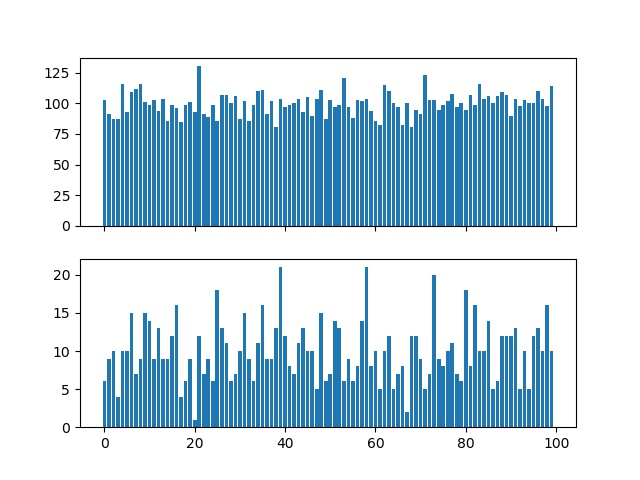
\includegraphics[scale=0.5]{graphs/a/1-Uniform.jpg}
                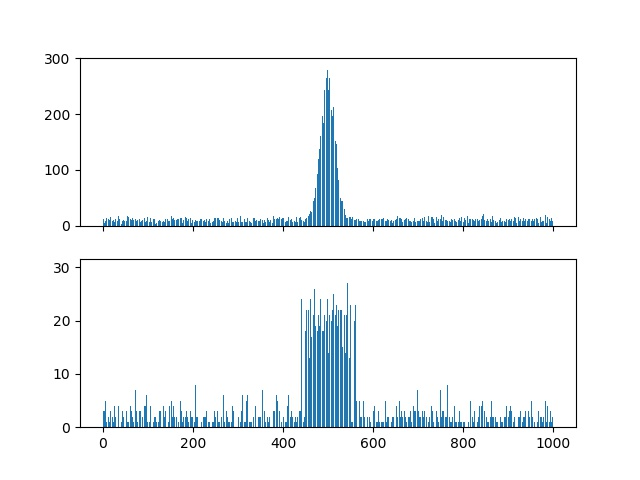
\includegraphics[scale=0.5]{graphs/a/1-Binomial.jpg}
            \end{center}
            For $\ell_{0}$ sampler performance in a turnstile or general stream, as the stream generated has an extremly large range, $\left[ 1,2^{16}-1 \right]$ but the total stream cannot be too long\footnote{The execution time is too long even for one update.}, the graph generated is trivial to see. However, an interesting observation from the results is that there is no failure during sampling even the sparsity $s$ grows to approximately $2k$ in the sampler.
        \subsection{Sparse Recovery}
            \subsubsection{1-Sparse Recovery}
                A sketch of execution result for 1-sparse structure under different sparsity in different streams with different sizes of unique items. Repeating this process did not cause oscillations in results, so randomly picking a output result is still representative.
                \begin{table}[h]
                    \centering
                    \begin{tabular}{|c|c|c|c|c|c|c|c|c|}
                    \hline
                                                     &                    & $s = 0$ & $s = 1$ & $s = 2$ & $s = 3$ & $s = 4$ & $s = 5$ & $s = 6$ \\ \hline
                    \multirow{2}{*}{$unique = 500$}  & \textbf{Turnstile} & 100     & 100     & 100     & 100     & 100     & 100     & 100     \\ \cline{2-9}
                                                     & \textbf{General}   & 100     & 99      & 100     & 100     & 100     & 99      & 99      \\ \hline
                    \multirow{2}{*}{$unique = 5000$} & \textbf{Turnstile} & 100     & 99      & 99      & 100     & 100     & 100     & 100     \\ \cline{2-9}
                                                     & \textbf{General}   & 100     & 99      & 100     & 99      & 100     & 100     & 99      \\ \hline
                    \end{tabular}
                \end{table}
            \subsubsection{$k$-Sparse Recovery}
                Similar to the previous table, the results did not vary too far in a sequence of consecutive executions. This is the lowest output picked from the results. It is a little bit confusing that the its ability to handle general streams is even better than strict turnstile stream. One of the possible justification is that a strict turnstile stream will always end up with non-negative frequencies for all numbers. Since a bigger number is likely to be factorised into more numbers which increases the probability of collisions, the difficulty of distinguishing between $k$-sparse and $(k+1)$-sparse grows significantly.
                \begin{table}[h]
                    \centering
                    \begin{tabular}{|c|c|c|c|c|c|c|c|c|}
                    \hline
                                                     &                    & $s = 0$ & $s = 1$ & $s = 2$ & $s = 3$ & $s = 4$ & $s = 5$ & $s = 6$ \\ \hline
                    \multirow{2}{*}{$unique = 500$}  & \textbf{Turnstile} & 100     & 98      & 94      & 70      & 90      & 95      & 100     \\ \cline{2-9}
                                                     & \textbf{General}   & 100     & 99      & 95      & 88      & 92      & 99      & 99      \\ \hline
                    \multirow{2}{*}{$unique = 5000$} & \textbf{Turnstile} & 100     & 99      & 92      & 68      & 75      & 94      & 99      \\ \cline{2-9}
                                                     & \textbf{General}   & 99      & 100     & 94      & 90      & 92      & 97      & 100     \\ \hline
                    \end{tabular}
                \end{table}
    \section{Future Improvement}
        It worths to see how pairwise independence improved the $\ell_{0}$ sampling metioned in \cite{Cormode:2014:UFA:2631033.2631080}. The initial design of the $\ell_{0}$ sampler uses an $\epsilon$-min-wise independent hash family, but the parameter $\epsilon$ was not considered in the generation of $k$-wise independent hash functions.
    \bibliographystyle{ieeetr}
    \bibliography{main}
\end{document}
